% WEMoE-NLP research report, following the Version 3 presentation. Build: latexmk -pdf main_v3.tex (pdfLaTeX + BibTeX).
% Preamble of theme-report/main.tex, reused unchanged (blank-line runs collapsed).
\documentclass[12pt, a4paper, oneside, final]{book} 
\usepackage{cmap}
\usepackage[unicode]{hyperref} 
\usepackage[utf8]{vietnam}
\usepackage{amsthm}
\usepackage{yhmath}
\usepackage{amsmath}
\usepackage{mathpazo}
\usepackage{booktabs}
% \usepackage{xcolor}

\usepackage{listings}
\usepackage{xcolor}

% Định nghĩa màu nền cho ô code
\definecolor{codegray}{rgb}{0.95,0.95,0.95}

\lstdefinestyle{pythonstyle}{
    language=Python,
    backgroundcolor=\color{codegray},
    basicstyle=\ttfamily\small,
    keywordstyle=\color{blue},
    stringstyle=\color{red},
    commentstyle=\color{green!60!black},
    showstringspaces=false,
    breaklines=true,
    frame=single,
    columns=flexible
}

\lstdefinestyle{sqlstyle}{
    language=SQL,
    basicstyle=\ttfamily\small,
    keywordstyle=\color{blue}\bfseries,
    commentstyle=\color{gray},
    stringstyle=\color{red!70!black},
    showstringspaces=false,
    breaklines=true,
    frame=single,
    columns=flexible
}

% \usepackage{arev}
% \usepackage[charter]{mathdesign}
% \usepackage[utopia]{mathdesign}
% \usepackage[mathscr]{eucal}
% \usepackage{fourier}
% \usepackage{charter}
% \usepackage{ccfonts} 
\usepackage{tasks}
\usepackage[dvipsnames]{xcolor}
\usepackage{tikz}
\usetikzlibrary{calc,angles}
\usetikzlibrary{intersections}
\usepackage{pgfplots}
\usepackage{indentfirst}
\usepackage{enumitem}
\usepackage{commath}
\usepackage{scrextend}
%%%%%%%%%%%%%%%%%%%%%%%%%%%%%%%%%%%%%%%%%%%
\usepackage{tikz,tkz-tab}
\usetikzlibrary{calc, angles, quotes, intersections, positioning, patterns}
\usepackage{pgfplots}
%%%%%%%%%%%%%%%%%%%%%%%%%%%%%%%%%%%%%%%%%%%
\usepackage{nicefrac}
\usepackage{picinpar}
% \usepackage{slashbox}
\usepackage{amssymb}
\usepackage{multicol} 
\usepackage{fancyhdr} 
\usepackage{graphicx}
\usepackage{geometry}
\usepackage{wrapfig}
\usepackage{multirow}
\usepackage{tabularx}
%\usepackage{standalone}%chen hinh bang file tex
%\usepackage{pstricks-add}
%\usepackage{pstricks,pst-plot,pst-text,pst-tree,pst-eps,pst-fill,pst-node,pst-math}

%\usepackage{mathptmx}  %Bổ sung thêm dòng này để dùng watermark
%\usepackage{draftwatermark} %Bổ sung thêm dòng này để dùng watermark

\geometry{left=2.5cm,right=1.5cm,top=2cm,bottom=2cm}

\setlength{\oddsidemargin}{-0.1in}
\setlength{\evensidemargin}{0.0in}
\setlength{\textwidth}{6.8in}
\setlength{\topmargin}{-0.5in}
\setlength{\textheight}{10.0in}
%%%%%%%%%%Mau moi
\colorlet{NAVYBLUE}{NavyBlue}
\usepackage{sectsty}
%\renewcommand{\thesection}{}

\sectionfont{\centering \fontsize{16}{16} \color{orange}\selectfont \scshape \MakeUppercase}

% Define rule (color) for header and footer
%\renewcommand{\headrule}{{\color{GreenYellow}\rule{\textwidth}{0.1pt}}} 
%\renewcommand{\footrule}{{\color{GreenYellow}\rule{\textwidth}{0.1pt}}} 
%%%%%%%%%%%%%%

\pagestyle{fancy} 
\fancyhead[L]{\texttt{}}
\fancyhead[R]{\texttt{\textcolor{NavyBlue} {\it }}} 
\fancyfoot[C]{} 
\fancyfoot[L]{ \textsf{\rightmark}}
\fancyfoot[R]{\textsf{\thepage}}
\renewcommand{\chaptermark}[1]{%
	\markboth{\chaptername\ \thechapter.\ #1}{}} %bỏ đi sẽ thấy chữ in
\renewcommand{\sectionmark}[1]{%
	\markright{\thesection.\ #1}} %bỏ đi sẽ thấy chữ in

\theoremstyle{definition} 
\newtheorem*{proposition}{\color{NavyBlue} Proposition}
\newtheorem*{definition}{\color{NavyBlue} Definition} 
\newtheorem{exercise}{\color{NavyBlue} Bài tập}[chapter] 
\newtheorem{bt}{\color{NavyBlue} Bài}[chapter]
%\newtheorem{exercise}{\color{blue} Bài tập}[chapter]
\newtheorem{tb}{\color{NavyBlue} Bảng}%[chapter]
\newtheorem{BT}{\color{NavyBlue} Bài toán}[chapter]
\newtheorem{vd}{\color{NavyBlue} Ví dụ}[chapter]
\newtheorem{dl}{\color{NavyBlue} Định lý}[chapter]
\newtheorem{nl}{\color{NavyBlue} Nguyên lý}[chapter]
\newtheorem{hq}{\color{NavyBlue} Hệ quả}[chapter]
\newtheorem{dn}{\color{NavyBlue} Định nghĩa}[chapter]
\newtheorem{tc}{\color{NavyBlue} Tính chất}[chapter]
\newtheorem{kn}{\color{NavyBlue} Khái niệm}[chapter]
\newtheorem{nx}{\color{NavyBlue} Nhận xét}[chapter]
\newtheorem{qt}{\color{NavyBlue} Quy tắc}[chapter]
\newtheorem{gt}{\color{NavyBlue} Giả thiết}[chapter]
\newtheorem{pl}{\color{NavyBlue} Phụ lục} %[chapter]
\newtheorem{cy}{\color{NavyBlue} Chú ý}[chapter]
\newcommand{\Lga}{\textcolor{NavyBlue}{\it Lời giải. \ }}
\newcommand{\Sol}{\textcolor{NavyBlue}{\it Lời giải. \  }}
\newcommand{\Gy}{\textcolor{NavyBlue}{\it Gợi ý. \  }}
\newcommand{\chm}{{\it Chứng minh. }}
\newcommand{\hd}{\textcolor{NavyBlue}{\it Hướng dẫn. }}
\newcommand{\ds}{\textcolor{NavyBlue}{\it \noindent Đáp số. }}
\newtheorem{example}{Ví dụ}[section]
\newcommand{\eproof}{\hfill $\square$}
\theoremstyle{plain} 
\newtheorem*{theorem}{Định lý}

\theoremstyle{remark} 
\newtheorem*{remark}{Chú ý}

\providecommand{\lr}[1]{\left( #1 \right)} 
\providecommand{\Lr}[1]{\left[ #1 \right]}
\providecommand{\LR}[1]{\left\{ #1 \right\}} 
\providecommand{\abs}[1]{\left\vert #1 \right\vert} 
\providecommand{\norm}[1]{\left\Vert #1 \right\Vert} 
\providecommand{\e}{\varepsilon} 
\providecommand{\Sum}[2]{\sum\limits_{#1}^{#2}} 
\providecommand{\Lim}{\lim\limits_{n \to +\infty}} 
\providecommand{\SUM}{\Sum{n = 1}{\infty}} 
\providecommand{\X}{\mathbb{X}}
\providecommand{\N}{\mathbb{N}}
\providecommand{\Z}{\mathbb{Z}}
\providecommand{\Q}{\mathbb{Q}}
\providecommand{\I}{\mathbb{I}}
\providecommand{\R}{\mathbb{R}}
\providecommand{\D}{\mathbb{D}}
\providecommand{\e}{\varepsilon}
\providecommand{\d}{\partial}
\providecommand{\ov}[1]{\overline{#1}} 
\providecommand{\al}[1]{\alpha{#1}} 
\providecommand{\ud}[1]{\underline{#1}} 

\DeclareMathSymbol{\INT}{\mathop}{largesymbols}{"5A} 
\renewcommand{\int}{\INT} 
\renewcommand{\iint}{\mathop{\int\!\!\!\!\!\int}}
\renewcommand{\iiint}{\mathop{\int\!\!\!\!\!\int\!\!\!\!\!\int}}
\DeclareMathOperator{\Int}{int} 
\DeclareMathOperator{\grad}{grad} 
\DeclareMathOperator{\sgn}{sgn} 
\providecommand{\hcn}{hình chữ nhật }
\DeclareMathOperator{\rank}{rank}
\DeclareMathOperator{\arccot}{arccot}
\DeclareMathOperator{\const}{const}
\DeclareMathOperator{\tg}{tg}
\DeclareMathOperator{\arctg}{arctg}
\DeclareMathOperator{\cotg}{cotg}
\DeclareMathOperator{\arccotg}{arccotg}
\DeclareMathOperator{\sh}{sh}
\DeclareMathOperator{\ch}{ch}
\DeclareMathOperator{\Sup}{Sup}
\DeclareMathOperator{\Inf}{Inf}
\DeclareMathOperator{\Min}{Min}
\DeclareMathOperator{\Max}{Max}

\newcounter{exerenumi}
\renewcommand{\theexerenumi}{\bf\alph{exerenumi}}
\newcommand{\labelexerenumi}{\theexerenumi.}
\newenvironment{answer}{\begin{list}{\labelexerenumi}{%
			\usecounter{exerenumi}%
			\setlength{\labelwidth}{3pt}%
			\setlength{\leftmargin}{0pt}%
			\setlength{\itemindent}{15pt}}}{\end{list}}
\def\baselinestretch{1.3}

\usepackage{fancyhdr}

\usepackage{xcolor}
\usepackage{sectsty}
\chapterfont{\color{NavyBlue}}  % sets colour of chapters
\sectionfont{\color{NavyBlue}}  % sets colour of sections
\subsectionfont{\color{NavyBlue}}  % sets colour of sections




% Additions to the theme: natbib is required by the theme's plainnat bibliography style.
\usepackage[numbers,sort&compress]{natbib}
\usepackage{url}
% Shared TikZ styles: NavyBlue comes from the report theme; the colour roles are constant across figures.
\usetikzlibrary{arrows.meta,fit,backgrounds,calc,positioning}
\tikzset{
  every node/.append style={font=\footnotesize\linespread{1}\selectfont},
  box/.style={rounded corners=1.5pt,align=center,inner sep=2.5pt,minimum height=.75cm},
  frz/.style={box,draw=NavyBlue,fill=NavyBlue!8},
  mix/.style={box,draw=BurntOrange,fill=Goldenrod!25,thick},
  trn/.style={box,draw=BrickRed,fill=BrickRed!14,thick},
  dat/.style={box,draw=black!50,fill=black!5},
  plain/.style={box,draw=none,fill=none},
  flow/.style={-{Latex[length=2mm]},thick,black!80},
  gate/.style={-{Latex[length=2mm]},thick,BrickRed},
  dict/.style={-{Latex[length=2mm]},thick,NavyBlue},
  group/.style={rounded corners=3pt,draw=black!45,dashed,inner sep=5pt},
  note/.style={font=\scriptsize\linespread{1}\selectfont,text=black!75,align=center},
  lane/.style={font=\footnotesize\bfseries,text=NavyBlue,anchor=west}
}
\newcommand{\figlegend}{%
  {\scriptsize\tikz\node[frz,minimum height=.22cm,minimum width=.35cm,inner sep=0]{};~frozen\quad
  \tikz\node[mix,minimum height=.22cm,minimum width=.35cm,inner sep=0]{};~input-conditioned\quad
  \tikz\node[trn,minimum height=.22cm,minimum width=.35cm,inner sep=0]{};~trainable during FSFT}}

\pgfplotsset{compat=1.18}
\graphicspath{{figures/}{figures_v3/}}
% Vietnamese document labels.
\AtBeginDocument{\renewcommand{\chaptername}{Chương}\renewcommand{\figurename}{Hình}\renewcommand{\tablename}{Bảng}\renewcommand{\bibname}{Tài liệu tham khảo}\renewcommand{\appendixname}{Phụ lục}}
\newcommand{\tablestyle}{\footnotesize\def\baselinestretch{1.05}\selectfont\renewcommand{\arraystretch}{1.12}\setlength{\tabcolsep}{4.5pt}\setlength{\belowcaptionskip}{4pt}}
\newcommand{\code}[1]{\texttt{\small #1}}
\newcommand{\figfont}{\fontsize{7}{8.4}\selectfont}
\hypersetup{pdftitle={Hợp nhất năm tác vụ NLP của GLUE bằng Weight-Ensembling Mixture of Experts},
  pdfauthor={Nguyễn Bá Anh; Nguyễn Thị Nhã Linh},colorlinks=true,linkcolor=NavyBlue,citecolor=NavyBlue,urlcolor=NavyBlue}
\setlength{\headheight}{15pt}
\setlength{\emergencystretch}{1.5em}
\hyphenation{WEMoE GLUE BERT}
% Tighter than the theme's 1.3 so that the main content fits the 15--20 page target.
\def\baselinestretch{1.03}
% Reduce the blank space above chapter titles.
\usepackage{etoolbox}
\makeatletter
% Each chapter starts on a new page, with a compact one-line heading.
\patchcmd{\chapter}{\thispagestyle{plain}}{}{}{\PatchFailed}
\renewcommand{\@makechapterhead}[1]{{\parindent\z@\raggedright\normalfont\LARGE\bfseries\color{NavyBlue}\@chapapp\space\thechapter.\space #1\par\nobreak\vskip 8\p@}}
\renewcommand{\@makeschapterhead}[1]{{\parindent\z@\raggedright\normalfont\LARGE\bfseries\color{NavyBlue}#1\par\nobreak\vskip 8\p@}}
\makeatother
% Let floats share pages with text instead of leaving gaps.
\renewcommand{\topfraction}{.9}\renewcommand{\bottomfraction}{.8}\renewcommand{\textfraction}{.1}\renewcommand{\floatpagefraction}{.75}

\begin{document}
\thispagestyle{empty}
\vspace*{4mm}

\noindent\textcolor{NavyBlue}{\rule{\linewidth}{1pt}}
\begin{center}
	\fontsize{26}{32} \color{NavyBlue} \selectfont
	\textbf{Hợp nhất năm tác vụ NLP của GLUE bằng Weight-Ensembling \mbox{Mixture of Experts}}
\end{center}

\noindent\textcolor{NavyBlue}{\rule{\linewidth}{1pt}}

\begin{center}
	\fontsize{17}{21} \selectfont
	Huấn luyện bộ định tuyến few-shot trên nền BERT dùng chung
\end{center}

\vspace*{2mm}
\begin{center}
	\fontsize{14}{14} \selectfont Báo cáo nghiên cứu
\end{center}
\vspace*{6mm}

\begin{center}
	\def\baselinestretch{1.0}\color{NavyBlue}
	{\fontsize{13}{13} \selectfont
		\begin{tabular}{l l}
			{\bf NHÓM THỰC HIỆN (NHÓM 1):} & \\[4mm]
			\hspace{13mm} NGUYỄN BÁ ANH & 20261218M\\[3mm]
			\hspace{13mm} NGUYỄN THỊ NHÃ LINH & 20261262M\\[6mm]
			{\bf GIẢNG VIÊN:} & \\[4mm]
			\hspace{13mm} NGUYỄN KIÊM HIẾU & \\[6mm]
			\hspace{13mm} Đại học Bách khoa Hà Nội & \\[3mm]
	\end{tabular}}
\end{center}


\newpage
\pagenumbering{arabic}
\renewcommand{\contentsname}{\color{NavyBlue}{MỤC LỤC}}
{\def\baselinestretch{0.88}\selectfont\small\tableofcontents}
\clearpage

\chapter*{Tóm tắt}
\addcontentsline{toc}{chapter}{Tóm tắt}
\markright{Tóm tắt}

Tinh chỉnh (fine-tuning) một mô hình ngôn ngữ huấn luyện trước (pre-trained) cho từng tác vụ mang lại hiệu năng tốt trên tác vụ đó, nhưng mỗi tác vụ mới lại thêm một mô hình hoàn chỉnh cần huấn luyện, lưu trữ và vận hành, đồng thời những gì học được cho một tác vụ không đến được các tác vụ khác. Nghiên cứu này xem xét liệu nhiều mô hình đã tinh chỉnh có thể trở thành một mô hình đa nhiệm duy nhất với trọng số thích ứng theo đầu vào hay không. Chúng tôi áp dụng Weight-Ensembling Mixture of Experts (WEMoE), vốn được đánh giá trên các vision Transformer, cho BERT và năm tác vụ nhị phân của bộ đánh giá GLUE: MRPC, RTE, CoLA, SST-2 và QNLI. Các trọng số ngoài khối MLP được hợp nhất tĩnh bằng Task Arithmetic, còn trọng số MLP của mỗi lớp encoder được dựng lại cho từng đầu vào bằng trọng số huấn luyện trước cộng với tổng các véc-tơ tác vụ đóng băng, theo hệ số do bộ định tuyến (router) quyết định. Chỉ các bộ định tuyến được huấn luyện, bằng Few-Shot Fine-Tuning (FSFT) trên các mẫu có nhãn mà các chuyên gia (expert) chưa từng thấy. Mọi lựa chọn mô hình đều dùng tập phát triển (dev), và điểm được báo cáo trên các tập kiểm định chính thức. Với 256 mẫu mỗi tác vụ, WEMoE đạt điểm trung bình $69.9\pm0.1$, so với 57.4 của Task Arithmetic, 78.2 của các chuyên gia và 45.8 của bộ dự đoán lớp đa số, tương ứng 59.1\% mức tăng giữa lớp đa số và các chuyên gia. Các hệ số không phụ thuộc đầu vào chỉ đạt $58.4\pm0.0$. Chỉ nâng cấp lớp đầu tiên của MLP cho điểm trung bình tương tự ($69.1\pm0.1$) với 47.2\% dung lượng lưu trữ của năm chuyên gia thay vì 73.1\%, nhưng hai biến thể yếu ở các tác vụ khác nhau. WEMoE không bằng chuyên gia ở tác vụ nào và chậm hơn nhiều lần khi chạy theo batch. Các hạn chế gồm một bộ chuyên gia duy nhất, tập kiểm định nhỏ ở hai tác vụ, và dữ liệu dev vượt quá ngân sách few-shot.

\vspace{3mm}
\noindent\textbf{Từ khóa:} hợp nhất mô hình; weight ensembling; Mixture of Experts; BERT; học đa nhiệm; few-shot fine-tuning.

\clearpage
\chapter{Bài toán}
\label{ch:problem}

\section{Vì sao mỗi tác vụ một mô hình riêng khó mở rộng}

Các mô hình ngôn ngữ huấn luyện trước (pre-trained) đã thay đổi cách xây dựng hệ thống xử lý ngôn ngữ tự nhiên. Một encoder như BERT~\cite{devlin2019bert} có thể được tinh chỉnh (fine-tune) cho một bài toán phân loại mới với lượng dữ liệu hạn chế, nên một hệ thống hỗ trợ nhiều tác vụ hiểu ngôn ngữ thường tích lũy một bản sao đã tinh chỉnh của cùng một kiến trúc cho mỗi tác vụ. Mỗi bản sao hoạt động tốt trên tác vụ của nó, nhưng cả tập hợp trở nên tốn kém theo bốn cách.

\begin{itemize}
  \item \textbf{Lưu trữ.} Mỗi bản sao giữ một bộ tham số hoàn chỉnh, dù tất cả đều xuất phát từ cùng một bộ trọng số huấn luyện trước.
  \item \textbf{Huấn luyện.} Mỗi tác vụ mới cần thêm một lần tinh chỉnh đầy đủ, với dữ liệu, tài nguyên tính toán và quy trình chọn mô hình riêng.
  \item \textbf{Vận hành.} Hệ thống phải quản lý phiên bản, nạp và chuyển yêu cầu đến một mô hình riêng cho từng tác vụ.
  \item \textbf{Cô lập kiến thức.} Mỗi mô hình chỉ biết tác vụ của nó. Những gì mô hình học được khi tinh chỉnh không đến được các mô hình khác.
\end{itemize}

\section{Phát biểu bài toán và câu hỏi nghiên cứu}
\label{sec:problem}

Gọi $\theta_0$ là trọng số của một mô hình huấn luyện trước, và $\theta_i$, $i\in\mathcal{T}$, là trọng số của các mô hình được tinh chỉnh từ nó cho một tập $\mathcal{T}$ gồm $T$ tác vụ. Chúng tôi gọi mỗi mô hình đã tinh chỉnh là một \emph{chuyên gia} (expert). \emph{Véc-tơ tác vụ} (task vector) của tác vụ $i$ là phần thay đổi mà quá trình tinh chỉnh tạo ra so với điểm xuất phát chung:
\begin{equation}
\tau_i=\theta_i-\theta_0 .
\label{eq:task-vector}
\end{equation}
Đầu vào của bài toán là $\theta_0$ cùng các trọng số $\theta_i$, hoặc tương đương là các véc-tơ tác vụ. Đầu ra là một mô hình đa nhiệm với trọng số $\theta_{\mathrm{mer}}=C(\theta_0,\theta_i)$, ánh xạ một văn bản và tác vụ của nó thành một nhãn. Bài toán là tìm hàm hợp nhất $C$ sao cho mô hình hợp nhất đạt ba mục tiêu:

\begin{enumerate}
  \item[\textbf{O1.}] Tích hợp kiến thức của các tác vụ một cách \emph{động}, tùy theo đầu vào.
  \item[\textbf{O2.}] Giữ chất lượng gần với các mô hình riêng theo tác vụ.
  \item[\textbf{O3.}] Cần ít tham số lưu trữ hơn so với việc giữ tất cả các mô hình.
\end{enumerate}

Không có ngưỡng đạt nào được đặt trước, nên ``gần'' được báo cáo như một khoảng cách đo được chứ không phải một kết quả đúng hoặc sai. Nghiên cứu này giải quyết bốn câu hỏi:

\begin{enumerate}
  \item[\textbf{RQ1.}] Các bộ định tuyến có thể khôi phục bao nhiêu hiệu năng bị mất do hợp nhất tĩnh, khi được huấn luyện trên các mẫu có nhãn mà các chuyên gia chưa từng thấy?
  \item[\textbf{RQ2.}] Mức khôi phục đó phụ thuộc vào ngân sách mẫu có nhãn như thế nào?
  \item[\textbf{RQ3.}] Cải thiện này có đòi hỏi định tuyến phụ thuộc đầu vào không, hay chỉ cần các hệ số cố định tốt hơn?
  \item[\textbf{RQ4.}] Việc chọn các lớp MLP để nâng cấp ảnh hưởng thế nào đến hành vi theo tác vụ và dung lượng lưu trữ, và phương pháp tốn bao nhiêu khi suy luận?
\end{enumerate}

\section{Vì sao bài toán quan trọng và vì sao khó}

\emph{Hợp nhất mô hình} (model consolidation), tức gộp các mô hình đã tinh chỉnh thành một, quan trọng vì nhiều hệ thống phục vụ các tác vụ ngôn ngữ có liên quan với nhau, và một mô hình chung giúp tái sử dụng kiến thức giữa chúng. Học đa nhiệm (multi-task learning)~\cite{caruana1997multitask} cũng tạo ra một mô hình, nhưng phải huấn luyện đồng thời trên toàn bộ dữ liệu và lặp lại chi phí đó khi thêm tác vụ. Hợp nhất mô hình bắt đầu từ các mô hình đã có, nên không cần huấn luyện chung lại từ đầu.

Cái khó nằm ở cách các mô hình đã tinh chỉnh khác biệt với nhau. Cập nhật có lợi cho tác vụ này có thể gây hại cho tác vụ khác khi cùng tác động lên một tham số, gọi là \emph{can nhiễu giữa các tác vụ}. Hai mô hình cũng có thể kéo một trọng số theo hai hướng ngược nhau, nên phép cộng làm mất một phần những gì mỗi mô hình đã học. Vì vậy, mọi phép hợp nhất đều phải quyết định giữ lại bao nhiêu từ mỗi cập nhật, và phải làm điều đó mà không có dữ liệu huấn luyện gốc của mọi tác vụ.

\section{Vì sao chỉ hợp nhất tĩnh có thể chưa đủ}

Một phương pháp tĩnh như Task Arithmetic~\cite{ilharco2023task} kết hợp tham số một lần và dùng một bộ trọng số cho mọi đầu vào. Năm tác vụ trong nghiên cứu này làm rõ giới hạn đó. Chúng đòi hỏi những điều khác nhau ở encoder: đánh giá ngữ pháp hoặc cảm xúc của một câu, hoặc xét quan hệ giữa hai câu qua diễn đạt lại, suy diễn hay trả lời câu hỏi. Một véc-tơ tham số duy nhất phải phục vụ tất cả cùng lúc, và hệ số tỉ lệ của nó chỉ có thể đánh đổi chúng với nhau. Như Tang và cộng sự~\cite{tang2024wemoe} lập luận, nghiệm tốt nhất có thể thay đổi theo đầu vào, nên một kết quả cố định khó có thể tốt nhất cho mọi tác vụ. Vì vậy, khoảng trống mà báo cáo này xem xét là liệu trọng số hợp nhất có nên thay đổi theo đầu vào thay vì cố định hay không.

\chapter{Ý tưởng}
\label{ch:idea}

\section{Mixture of Experts: khái niệm cốt lõi}

Mixture of Experts (MoE)~\cite{jacobs1991adaptive,shazeer2017moe,mu2025survey} giải quyết bài toán bằng nhiều mạng chuyên biệt $E_1,\dots,E_n$ và một mạng nhỏ gọi là \emph{bộ định tuyến} (router) hay cổng, $G$, quyết định mỗi chuyên gia được tính bao nhiêu cho đầu vào hiện tại (Hình~\ref{fig:moe}):
\begin{equation}
\mathrm{MoE}(x)=C\big(\{G_i(x)\cdot E_i(x)\}_{i=1}^{n}\big),
\label{eq:moe}
\end{equation}
trong đó $G_i(x)$ là mức đóng góp của chuyên gia $i$ và $C$ là một hàm kết hợp, theo cách cổ điển là phép cộng. Vì $G$ nhận $x$ làm đầu vào, mức đóng góp thay đổi từ đầu vào này sang đầu vào khác. Đây chính là hành vi động mà mục tiêu O1 yêu cầu.

\begin{figure}[htbp]
  \centering
  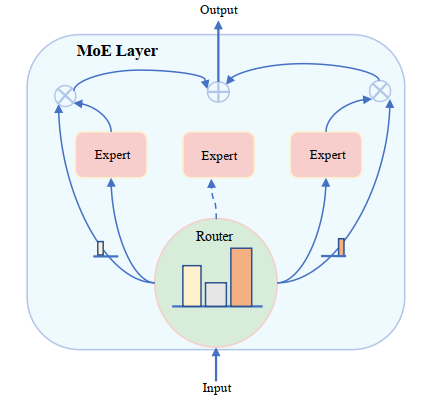
\includegraphics[width=.38\linewidth]{arch_moe.png}
  \caption{Một lớp Mixture of Experts, theo Mu và Lin~\cite{mu2025survey}. Bộ định tuyến đặt mức đóng góp của mỗi chuyên gia cho đầu vào hiện tại.}
  \label{fig:moe}
\end{figure}

\section{Từ kết hợp đầu ra đến kết hợp trọng số}

Phương trình~\eqref{eq:moe} kết hợp \emph{đầu ra} của các chuyên gia. Nếu áp dụng trực tiếp, mọi chuyên gia phải chạy cho mọi đầu vào, nên chi phí suy luận tăng theo số chuyên gia và các chuyên gia cần một không gian đầu ra chung. Weight-Ensembling Mixture of Experts (WEMoE)~\cite{tang2024wemoe} giữ bộ định tuyến nhưng thay đổi đối tượng được kết hợp. Mỗi chuyên gia được biểu diễn bằng véc-tơ tác vụ của nó, giá trị của bộ định tuyến nhân vào các véc-tơ đó, và trọng số kết quả được dựng lên trước khi áp dụng (Hình~\ref{fig:we}).

Hai cách này không tương đương. Với một lớp tuyến tính, $(\sum_i w_iW_i)h=\sum_i w_i(W_ih)$, nhưng đẳng thức này không còn đúng qua các hàm kích hoạt phi tuyến và các lớp xếp chồng. Do đó, kết hợp trọng số định nghĩa một hàm khác với tổ hợp đầu ra của các chuyên gia. Lợi ích tiềm năng của nó là một lượt truyền xuôi (forward pass) cho mỗi đầu vào, một checkpoint và một encoder dùng chung. Chi phí của nó là véc-tơ tác vụ phải được lưu cho mọi mô-đun nâng cấp, bộ định tuyến cần dữ liệu để huấn luyện, và mỗi đầu vào cần dựng trọng số riêng lúc chạy, điều này có thể làm suy luận chậm hơn ngay cả khi lưu ít tham số hơn. Mục~\ref{sec:efficiency} đo các chi phí này.

\begin{figure}[htbp]
  \centering
  \resizebox{.62\linewidth}{!}{\input{figures_vi/weight_ensembling}}
  \caption{Kết hợp ở mức tham số được dùng trong nghiên cứu này (a), đối chiếu với kết hợp ở mức đầu ra (b), chỉ được vẽ để tham khảo.}
  \label{fig:we}
\end{figure}

\section{Luồng thực hiện: từ dữ liệu đến đánh giá}
\label{sec:flow}

Hình~\ref{fig:flow} cho thấy luồng thực hiện gồm bốn chặng. Chặng 1 chuẩn bị năm tác vụ GLUE và chia mỗi tập huấn luyện chính thức thành ba phần. Chặng 2 tinh chỉnh một chuyên gia cho mỗi tác vụ từ mô hình huấn luyện trước, rồi giữ lại véc-tơ tác vụ và đầu phân loại (head) của nó. Chặng 3 hợp nhất chúng thành một mô hình và huấn luyện các bộ định tuyến trên tập few-shot. Chặng 4 báo cáo điểm trên các tập kiểm định chính thức, cùng dung lượng lưu trữ và độ trễ. Tập phát triển chọn epoch tốt nhất, hệ số tỉ lệ $\lambda$ và bước tốt nhất của bộ định tuyến, nên không lựa chọn nào chạm vào dữ liệu được báo cáo. Trọng số chuyên gia được đóng băng sau Chặng 2, và chỉ các bộ định tuyến học ở Chặng 3.

\begin{figure}[htbp]
  \centering
  \resizebox{.8\linewidth}{!}{\input{figures_v3_vi/flow}}
  \caption{Luồng thực hiện: từ dữ liệu đến đánh giá. Mũi tên nét đứt cho biết nơi tập phát triển chọn mô hình. $\theta_i$ và $\tau_i$ được định nghĩa ở Mục~\ref{sec:problem}, $g_i$ là head của chuyên gia $i$, và $\lambda$ là hệ số tỉ lệ của Task Arithmetic ở Mục~\ref{sec:ta}.}
  \label{fig:flow}
\end{figure}

\chapter{Lý thuyết và phương pháp: WEMoE}
\label{ch:theory}

Trong chương này, $T=5$ là số tác vụ và số chuyên gia, $i$ là chỉ số chuyên gia, $t$ là tác vụ của một đầu vào, $\ell\in\{1,\dots,12\}$ là chỉ số lớp encoder, và $j$ là chỉ số của $N$ token trong một đầu vào. Phương pháp được mô tả đúng như đã cài đặt trong nghiên cứu này.

\section{Encoder BERT và phần xương sống dùng chung}

BERT~\cite{devlin2019bert} là một Transformer~\cite{vaswani2017attention} chỉ gồm encoder. Mô hình được dùng ở đây là \texttt{bert-base-uncased}, với 12 lớp encoder, kích thước ẩn $d=768$, 12 đầu attention và kích thước MLP 3072, tổng cộng 109.5M tham số cho mỗi chuyên gia, kể cả head. Hình~\ref{fig:bert} cho thấy cấu trúc này. Token được ánh xạ thành tổng của embedding token, embedding đoạn và embedding vị trí, sau đó là chuẩn hóa lớp (layer normalisation)~\cite{ba2016layernorm}. Mỗi lớp encoder có hai lớp con. Self-attention cho mỗi token một trạng thái phản ánh toàn bộ ngữ cảnh, liên hệ các truy vấn $Q$ với các khóa $K$ có số chiều $d_k$ và các giá trị $V$:
\begin{equation}
\mathrm{Attention}(Q,K,V)=\mathrm{softmax}\!\left(\frac{QK^{\top}}{\sqrt{d_k}}\right)V .
\label{eq:attention}
\end{equation}
Lớp con thứ hai là mạng truyền thẳng theo vị trí, ở đây gọi là \emph{khối MLP}:
\begin{equation}
\mathrm{MLP}(h)=W_2\,\mathrm{GELU}(W_1h+b_1)+b_2 ,
\label{eq:ffn}
\end{equation}
trong đó $h$ là trạng thái của một token, GELU là hàm kích hoạt của Hendrycks và Gimpel~\cite{hendrycks2016gelu}, còn $(W_1,b_1)$ và $(W_2,b_2)$ là lớp tuyến tính thứ nhất và thứ hai của khối, gọi là fc1 và fc2. Mỗi lớp con được bọc theo dạng $h'=\mathrm{LayerNorm}\big(h+\mathrm{Sublayer}(h)\big)$. Để phân loại, trạng thái \texttt{[CLS]} cuối cùng đi qua pooler, là một lớp dense với $\tanh$, rồi đến head riêng của tác vụ $g_t$, gồm dropout và một lớp tuyến tính có hai đầu ra. Mọi chuyên gia xuất phát từ cùng một bộ trọng số và có chung cấu trúc này, nên trọng số của chúng có thể được trừ và cộng theo từng vị trí.

\begin{figure}[htbp]
  \centering
  \resizebox{.82\linewidth}{!}{\input{figures_v3_vi/bert}}
  \caption{Encoder BERT dùng trong nghiên cứu này, từ token đầu vào đến logit (trên), với một lớp encoder được phóng to (dưới). Các lớp dropout không được vẽ.}
  \label{fig:bert}
\end{figure}

\section[Kiến trúc WEMoE: hợp nhất tĩnh và phụ thuộc đầu vào]{Kiến trúc WEMoE: hợp nhất tĩnh và\\ phụ thuộc đầu vào}

WEMoE chia tham số thành hai nhóm. Trong thiết kế của Tang và cộng sự~\cite{tang2024wemoe}, thể hiện ở Hình~\ref{fig:overview}, attention và chuẩn hóa lớp được hợp nhất tĩnh, còn mỗi MLP được ``nâng cấp'' (upscale) thành một mô-đun Weight-Ensembling MoE, nghĩa là trọng số của nó trở thành phụ thuộc đầu vào. Các vision Transformer của họ chuẩn hóa trước mỗi lớp con. BERT chuẩn hóa sau lớp con, nên Hình~\ref{fig:arch} thể hiện cùng nguyên lý như đã cài đặt trên BERT. Ở đây, nhóm tĩnh là mọi trọng số của encoder ngoài các lớp được nâng cấp, kể cả embedding và pooler. Bảng~\ref{tab:components} liệt kê các thành phần, trong đó $W_0^{\ell}$ và $\tau_i^{\ell}$ là phần của $\theta_0$ và $\tau_i$ thuộc MLP của lớp $\ell$, $\lambda$ là hệ số tỉ lệ ở Mục~\ref{sec:ta} và $r^{\ell}$ là bộ định tuyến ở Mục~\ref{sec:router}. Bộ định tuyến chỉ thấy trạng thái token và không nhận mã tác vụ (task id); mã này chỉ dùng để chọn head.

\begin{figure}[htbp]
  \centering
  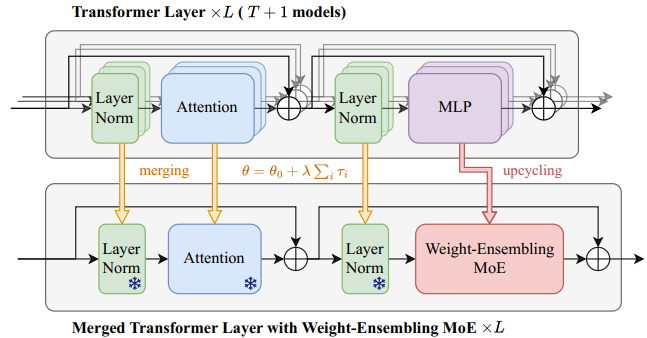
\includegraphics[width=.38\linewidth]{arch_wemoe_overview.png}
  \caption{Thiết kế WEMoE gốc trên vision Transformer chuẩn hóa trước, theo Tang và cộng sự~\cite{tang2024wemoe}. Trên: các mô hình đã tinh chỉnh và mô hình huấn luyện trước. Dưới: lớp đã hợp nhất. Các phần đóng băng có dấu bông tuyết.}
  \label{fig:overview}
\end{figure}

\begin{figure}[htbp]
  \centering
  \resizebox{.76\linewidth}{!}{\input{figures_v3_vi/architecture}}\\[2pt]
  {\scriptsize\tikz\node[frz,minimum height=.22cm,minimum width=.35cm,inner sep=0]{};~đóng băng\quad
  \tikz\node[mix,minimum height=.22cm,minimum width=.35cm,inner sep=0]{};~phụ thuộc đầu vào\quad
  \tikz\node[trn,minimum height=.22cm,minimum width=.35cm,inner sep=0]{};~huấn luyện trong FSFT}
  \caption{Mô hình WEMoE hợp nhất như đã cài đặt. Trong phạm vi full, cả fc1 và fc2 đều phụ thuộc đầu vào. Trong phạm vi intermediate-only, fc2 là tĩnh và dùng Task Arithmetic.}
  \label{fig:arch}
\end{figure}

\begin{table}[htbp]
  \centering\tablestyle
  \caption{Các thành phần của mô hình hợp nhất trong biến thể mặc định full MLP.}
  \label{tab:components}
  \begin{tabularx}{\linewidth}{l X c}
    \toprule
    Thành phần & Nguồn gốc & Trong FSFT\\
    \midrule
    Embedding, attention, chuẩn hóa lớp, pooler & Task Arithmetic với $\lambda$ chọn trên dev & Đóng băng\\
    Trọng số MLP gốc $W_0^{\ell}$ & Mô hình huấn luyện trước & Đóng băng\\
    Véc-tơ tác vụ của MLP $\tau_i^{\ell}$ & Chuyên gia trừ mô hình huấn luyện trước & Đóng băng\\
    Các head phân loại $g_t$ & Mỗi chuyên gia một head & Đóng băng\\
    Các bộ định tuyến $r^{\ell}$ & Mới, mỗi lớp encoder một bộ & \textbf{Huấn luyện}\\
    \bottomrule
  \end{tabularx}
\end{table}

Cách phân chia này quyết định chi phí lưu trữ. Phần tĩnh được lưu một lần. Mỗi lớp được nâng cấp phải giữ trọng số huấn luyện trước và một véc-tơ tác vụ cho mỗi chuyên gia, tức là $T+1$ bản của lớp đó, và các bộ định tuyến thêm tham số $\phi$ của riêng chúng:
\begin{equation}
|\theta_{\mathrm{static}}|+(T+1)\,|\theta_{\mathrm{MLP}}|+|\phi|+|\mathrm{heads}|,
\label{eq:storage}
\end{equation}
trong đó $\theta_{\mathrm{MLP}}$ là các lớp được nâng cấp. Chúng tôi đánh giá hai phạm vi: \emph{full}, nâng cấp fc1 và fc2, và \emph{intermediate-only}, chỉ nâng cấp fc1. Các véc-tơ tác vụ chiếm phần lớn tham số lưu trữ của phạm vi full (Bảng~\ref{tab:storage}), nên mức tiết kiệm phụ thuộc mạnh vào lựa chọn này. Tang và cộng sự chọn MLP dựa trên quan sát trên các mô hình CLIP-ViT rằng trọng số attention giữ hướng gần với mô hình huấn luyện trước hơn trọng số MLP. Chúng tôi không lặp lại phép đo đó trên BERT, nên lựa chọn này là kế thừa chứ chưa được kiểm chứng độc lập ở đây.

\section{Task Arithmetic và véc-tơ tác vụ}
\label{sec:ta}

Véc-tơ tác vụ (Phương trình~\ref{eq:task-vector}) ghi lại những gì tinh chỉnh đã thay đổi cho một tác vụ. Task Arithmetic~\cite{ilharco2023task} cộng các véc-tơ này vào mô hình gốc với một hệ số tỉ lệ $\lambda$:
\begin{equation}
\theta=\theta_0+\lambda\sum_{i=1}^{T}\tau_i .
\label{eq:ta}
\end{equation}
Simple Averaging là trường hợp đặc biệt $\lambda=1/T$, bằng trung bình trọng số của các chuyên gia. $\lambda$ nhỏ giữ mô hình gần mô hình huấn luyện trước, còn $\lambda$ lớn áp dụng các cập nhật mạnh hơn, kể cả những xung đột giữa chúng. Chúng tôi chọn $\lambda$ bằng tìm kiếm lưới theo điểm dev trung bình (Mục~\ref{sec:merging}). Phương pháp này đơn giản và không thêm tham số, nhưng kết quả giống nhau với mọi đầu vào.

\section{Bộ định tuyến và MLP phụ thuộc đầu vào}
\label{sec:router}

Mỗi lớp encoder có bộ định tuyến riêng $r^{\ell}$ (Hình~\ref{fig:router}). Đầu vào của nó là chuỗi trạng thái token $h^{\ell}_j\in\mathbb{R}^{d}$ ra khỏi Add\&Norm thứ nhất của lớp đó. Bộ định tuyến có hai lớp tuyến tính với ReLU và được áp dụng cho từng token:
\begin{equation}
r^{\ell}(h)=A^{\ell}_2\,\mathrm{ReLU}\big(A^{\ell}_1h+c^{\ell}_1\big)+c^{\ell}_2,
\label{eq:router}
\end{equation}
với $A^{\ell}_1\in\mathbb{R}^{d\times d}$ và $A^{\ell}_2\in\mathbb{R}^{T\times d}$. Mười hai bộ định tuyến có $12\,(d^2+d+Td+T)=7\,133\,244$ tham số huấn luyện được. Đầu ra theo token được lấy trung bình trên các vị trí không phải padding, dùng mặt nạ attention $m_j\in\{0,1\}$, để có một véc-tơ cho mỗi đầu vào, nên padding không ảnh hưởng đến định tuyến:
\begin{equation}
w^{\ell}(x)=\frac{\sum_j m_j\,r^{\ell}(h^{\ell}_j)}{\sum_j m_j}\in\mathbb{R}^{T}.
\label{eq:gating}
\end{equation}
Với đầu vào $x$, mỗi lớp tuyến tính được nâng cấp được dựng lại từ trọng số huấn luyện trước và phần tương ứng của các véc-tơ tác vụ, và bias cũng được dựng lại theo cách tương tự:
\begin{equation}
W^{\ell}(x)=W_0^{\ell}+\sum_{i=1}^{T}w_i^{\ell}(x)\,\tau_i^{\ell},\qquad
b^{\ell}(x)=b_0^{\ell}+\sum_{i=1}^{T}w_i^{\ell}(x)\,\tau_i^{\ell,b}.
\label{eq:we}
\end{equation}
Hai lớp tuyến tính của một khối dùng chung $w^{\ell}(x)$. Dự đoán dùng head $g_t$ của tác vụ đã biết, trong đó $\bar\theta$ là các trọng số hợp nhất tĩnh:
\begin{equation}
p(y\mid x,t)=\mathrm{softmax}\Big(g_t\big(\mathrm{pool}(\mathrm{BERT}(x;\bar\theta,\{W^{\ell}(x)\}))\big)\Big),\quad
\hat y=\arg\max_{y}\,p(y\mid x,t).
\label{eq:prediction}
\end{equation}

\begin{figure}[htbp]
  \centering
  \begin{minipage}[c]{.25\linewidth}\centering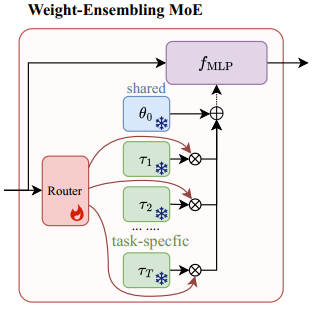
\includegraphics[width=\linewidth]{arch_wemoe_module.png}\end{minipage}\hfill
  \begin{minipage}[c]{.72\linewidth}\centering\resizebox{\linewidth}{!}{\input{figures_vi/router}}\end{minipage}
  \caption{Trái: mô-đun WEMoE của Tang và cộng sự~\cite{tang2024wemoe}. Phải: bộ định tuyến của lớp $\ell$ như đã cài đặt, áp dụng cho từng token và lấy trung bình trên các token không phải padding.}
  \label{fig:router}
\end{figure}

Các giá trị của bộ định tuyến \emph{không được chuẩn hóa}. Không có softmax và không chọn top-$k$, nên một giá trị có thể lớn hơn 1 hoặc âm, tức là bộ định tuyến có thể khuếch đại hoặc trừ đi một véc-tơ tác vụ, và phép kết hợp không lồi cũng không thưa. Trọng số tuyến tính được khởi tạo từ $\mathcal{N}(0,0.01^2)$ với $c^{\ell}_1=0$ và $c^{\ell}_2=\lambda$, nên $w^{\ell}_i(x)\approx\lambda$ lúc bắt đầu và mô hình xuất phát gần Task Arithmetic. Các unit test trên mô hình ngẫu nhiên nhỏ xác nhận rằng định tuyến hằng bằng Task Arithmetic, padding không ảnh hưởng đến định tuyến và chỉ các bộ định tuyến nhận gradient.

\section{Hàm mục tiêu Few-Shot Fine-Tuning (FSFT)}
\label{sec:fsft}

Các bộ định tuyến được huấn luyện bằng Few-Shot Fine-Tuning: cross-entropy trên một tập nhỏ có nhãn, cộng qua các tác vụ. Với mỗi tác vụ, $k$ mẫu $D_t^{(k)}$ được lấy từ một tập dự trữ, và với seed cố định thì $k$ nhỏ hơn cho một tập con của $k$ lớn hơn. Ở mỗi bước, một mini-batch $B_t$ được lấy cho mỗi tác vụ, và hàm mục tiêu là
\begin{equation}
\min_{\phi}\ \sum_{t=1}^{T}\ \frac{1}{|B_t|}\sum_{(x,y)\in B_t}-\log p_{\phi}(y\mid x,t),
\qquad B_t\subset D_t^{(k)},\ \ |D_t^{(k)}|=k ,
\label{eq:fsft}
\end{equation}
trong đó $p_\phi$ là phân phối của Phương trình~\eqref{eq:prediction}. Mọi thành phần ngoài $\phi$ được giữ đóng băng, và dropout bị tắt. Điểm dev trung bình được đánh giá trước khi huấn luyện và sau mỗi 50 bước, và trạng thái bộ định tuyến ở bước tốt nhất được khôi phục khi kết thúc. Vì vậy, một lần chạy có bước tốt nhất bằng 0 sẽ báo cáo bộ định tuyến chưa huấn luyện.

Bảng~\ref{tab:comparison} phân biệt phương pháp gốc với nghiên cứu này. Khác biệt lớn nhất là hàm mục tiêu. Tang và cộng sự tối thiểu hóa entropy của dự đoán trên dữ liệu kiểm thử không nhãn, tức là thích ứng lúc kiểm thử (test-time adaptation), và hàm mục tiêu này không được dùng ở đây. FSFT dùng các mẫu huấn luyện có nhãn và không bao giờ chạm vào tập dùng để báo cáo. Do đó, kết quả của hai nghiên cứu không so sánh trực tiếp được.

\begin{table}[htbp]
  \centering\tablestyle
  \caption{Nghiên cứu WEMoE gốc của Tang và cộng sự~\cite{tang2024wemoe} và nghiên cứu này.}
  \label{tab:comparison}
  \begin{tabularx}{\linewidth}{>{\bfseries\raggedright\arraybackslash}p{3.1cm} *{2}{>{\raggedright\arraybackslash}X}}
    \toprule
    Khía cạnh & Tang và cộng sự & Nghiên cứu này\\
    \midrule
    Backbone, tác vụ & Các mô hình thị giác CLIP-ViT; tám tác vụ phân loại ảnh & BERT-base; năm tác vụ nhị phân của GLUE\\
    Huấn luyện bộ định tuyến & Thích ứng lúc kiểm thử: entropy trên dữ liệu kiểm thử không nhãn & FSFT: cross-entropy trên $k$ mẫu có nhãn mỗi tác vụ\\
    Đầu vào định tuyến & Trung bình trên các token & Trung bình trên các token không phải padding\\
    Mô-đun được nâng cấp & Các MLP của Transformer & Full MLP; intermediate-only là ablation\\
    \bottomrule
  \end{tabularx}
\end{table}

\chapter{Phương pháp thực nghiệm}
\label{ch:method}

\section{Năm tác vụ nhị phân của GLUE và dữ liệu}

Thực nghiệm dùng năm tác vụ nhị phân của bộ đánh giá General Language Understanding Evaluation (GLUE)~\cite{wang2019glue}, được nạp qua thư viện Hugging Face Datasets~\cite{lhoest2021datasets} và liệt kê trong Bảng~\ref{tab:data}: MRPC~\cite{dolan2005mrpc}, RTE~\cite{dagan2006rte}, CoLA~\cite{warstadt2019cola}, SST-2~\cite{socher2013sst} và QNLI, được xây dựng từ SQuAD~\cite{rajpurkar2016squad}. CoLA và SST-2 nhận một câu, còn MRPC, RTE và QNLI nhận một cặp. Đầu vào được tách token và cắt còn tối đa 128 token. Các tác vụ khác nhau nhiều về kích thước, như Bảng~\ref{tab:split} cho thấy, và về điểm mà một dự đoán hằng đạt được, như cột cuối của Bảng~\ref{tab:data} cho thấy.

\begin{table}[htbp]
  \centering\tablestyle
  \caption{Năm tác vụ GLUE. ``Đa số \%'' là độ chính xác trên tập kiểm định khi luôn dự đoán nhãn phổ biến nhất.}
  \label{tab:data}
  \setlength{\tabcolsep}{3.5pt}\begin{tabularx}{\linewidth}{l X l l l r}
    \toprule
    Tác vụ & Xác định liệu\ldots & Trường đầu vào & Nhãn & Độ đo & Đa số \%\\
    \midrule
    MRPC & hai câu có cùng nghĩa & sentence1, sentence2 & not\_equivalent / equivalent & acc + F1 & 68.4\\
    RTE & một câu suy ra được câu kia & sentence1, sentence2 & entailment / not\_entailment & accuracy & 52.7\\
    CoLA & một câu đúng ngữ pháp & sentence & unacceptable / acceptable & MCC & 69.1\\
    SST-2 & một câu tích cực hay tiêu cực & sentence & negative / positive & accuracy & 50.9\\
    QNLI & một câu trả lời được câu hỏi & question, sentence & entailment / not\_entailment & accuracy & 50.5\\
    \bottomrule
  \end{tabularx}
\end{table}

\section{Chia dữ liệu và quy trình thực nghiệm}
\label{sec:protocol}

Tập huấn luyện chính thức của mỗi tác vụ được hoán vị một lần với seed 42 và chia thành ba phần rời nhau (Bảng~\ref{tab:split}). Vì vậy, bốn loại dữ liệu có vai trò riêng biệt:

\begin{itemize}
  \item \textbf{Dữ liệu huấn luyện chuyên gia} là phần còn lại sau hai phần dự trữ bên dưới. Chỉ các chuyên gia huấn luyện trên phần này.
  \item \textbf{Tập few-shot} (few-shot pool) gồm 256 mẫu có nhãn mỗi tác vụ, và $k$ mẫu trong đó huấn luyện các bộ định tuyến. Các chuyên gia không bao giờ thấy tập này.
  \item \textbf{Tập phát triển} (dev) bằng 10\% tập huấn luyện chính thức, tối đa 1\,000 mẫu. Mọi lựa chọn đều dựa vào tập này: epoch của chuyên gia, $\lambda$ và bước FSFT.
  \item \textbf{Tập kiểm định chính thức} (official validation) chỉ dùng cho điểm được báo cáo.
\end{itemize}

Các tập kiểm thử của GLUE không được dùng. Nhãn của chúng bị ẩn trong dữ liệu ở bốn tác vụ, và nhãn kiểm thử của MRPC cũng không được sử dụng. Quy trình này ngăn các dạng rò rỉ dữ liệu chính, nhưng có chi phí: RTE, tác vụ nhỏ nhất, chỉ còn 1\,985 trong 2\,490 cặp huấn luyện cho chuyên gia của nó.

\begin{table}[htbp]
  \centering\tablestyle
  \caption{Cách chia dữ liệu theo tác vụ. Dòng cuối ghi mục đích sử dụng của từng tập.}
  \label{tab:split}
  \begin{tabular}{l r r r r r}
    \toprule
    Tác vụ & Train chính thức & Tập few-shot & Dev & Train chuyên gia & Kiểm định chính thức\\
    \midrule
    MRPC & 3\,668 & 256 & 367 & 3\,045 & 408\\
    RTE & 2\,490 & 256 & 249 & 1\,985 & 277\\
    CoLA & 8\,551 & 256 & 855 & 7\,440 & 1\,043\\
    SST-2 & 67\,349 & 256 & 1\,000 & 66\,093 & 872\\
    QNLI & 104\,743 & 256 & 1\,000 & 103\,487 & 5\,463\\
    \midrule
    \textbf{Dùng cho} & & \textbf{FSFT} & \textbf{Lựa chọn} & \textbf{Chuyên gia} & \textbf{Báo cáo}\\
    \bottomrule
  \end{tabular}
\end{table}

\section{Huấn luyện năm chuyên gia}

Mỗi chuyên gia tinh chỉnh mọi lớp của \texttt{bert-base-uncased} và một head hai lớp mới bằng cross-entropy trên dữ liệu huấn luyện chuyên gia của nó. Cả năm dùng chung một công thức, ở cột đầu của Bảng~\ref{tab:config}, không tinh chỉnh riêng theo tác vụ, và epoch tốt nhất trong ba epoch được chọn trên dev theo điểm tác vụ. AdamW~\cite{loshchilov2019adamw} chỉ áp dụng weight decay cho các tham số có ít nhất hai chiều.

\begin{table}[htbp]
  \centering\tablestyle
  \caption{Cấu hình huấn luyện của hai giai đoạn tối ưu.}
  \label{tab:config}
  \begin{tabularx}{\linewidth}{>{\bfseries}l *{2}{>{\raggedright\arraybackslash}X}}
    \toprule
    Thiết lập & Chuyên gia theo tác vụ & FSFT (bộ định tuyến)\\
    \midrule
    Tham số huấn luyện được & Toàn bộ BERT và head (109.5M mỗi chuyên gia) & Chỉ bộ định tuyến (7.1M); 60 ở biến thể không phụ thuộc đầu vào\\
    Bộ tối ưu & AdamW; weight decay 0.01 & AdamW; không weight decay\\
    Learning rate & $2\times10^{-5}$ & $10^{-4}$; $10^{-3}$ ở biến thể không phụ thuộc đầu vào\\
    Lịch học & Tuyến tính, warmup 10\% & Tuyến tính, warmup 10\%\\
    Batch size, thời lượng & 32; 3 epoch & 16 mỗi tác vụ; 500 bước\\
    Cắt gradient & Chuẩn 1.0 & Không\\
    Lựa chọn trên dev & Epoch tốt nhất theo điểm tác vụ & Bước tốt nhất theo điểm trung bình, mỗi 50 bước\\
    \bottomrule
  \end{tabularx}
\end{table}

\section{Hợp nhất các chuyên gia và huấn luyện bộ định tuyến với dữ liệu few-shot}
\label{sec:merging}

Task Arithmetic chọn $\lambda$ từ $\{0.1,0.2,\dots,1.0\}$ theo điểm dev trung bình (Bảng~\ref{tab:lambda}). Điểm đạt đỉnh tại $\lambda=0.3$, và giá trị này khởi tạo các mô hình hợp nhất. Tập dev có thể gây hiểu nhầm với mô hình hợp nhất trên SST-2: tại $\lambda=0.3$, Task Arithmetic đạt 83.7 trên dev nhưng chỉ 69.8 trên tập kiểm định. Hai tập này khác nhau về bản chất, vì văn bản huấn luyện của SST-2 trung bình dài 9.4 từ còn văn bản kiểm định dài 19.5 từ. Chọn trên dev vẫn là quy trình đúng, nhưng điểm dev của SST-2 đánh giá cao hơn thực tế chất lượng của mô hình hợp nhất.

\begin{table}[htbp]
  \centering\tablestyle
  \caption{Điểm dev của Task Arithmetic trên lưới $\lambda$ ($\times100$).}
  \label{tab:lambda}
  \begin{tabular}{l c c c c c c c c c c}
    \toprule
    $\lambda$ & 0.1 & 0.2 & \textbf{0.3} & 0.4 & 0.5 & 0.6 & 0.7 & 0.8 & 0.9 & 1.0\\
    \midrule
    Điểm dev trung bình & 52.0 & 57.4 & \textbf{62.8} & 60.7 & 58.6 & 58.0 & 57.5 & 57.3 & 57.4 & 57.1\\
    Điểm dev SST-2 & 62.4 & 73.3 & \textbf{83.7} & 89.8 & 91.7 & 92.3 & 93.0 & 93.2 & 92.9 & 92.5\\
    \bottomrule
  \end{tabular}
\end{table}

Mười lăm lần chạy FSFT đã được thực hiện, ba seed cho mỗi trong năm cấu hình. Mô hình chính là WEMoE \emph{full MLP} với $k\in\{16,64,256\}$. Hai \emph{ablation}, tức thí nghiệm thay đổi một thành phần và giữ nguyên phần còn lại, dùng $k=256$. Biến thể \emph{intermediate-only} chỉ nâng cấp fc1, còn fc2 dùng Task Arithmetic. Biến thể \emph{không phụ thuộc đầu vào} (input-independent) không có bộ định tuyến: nó học một hệ số cho mỗi chuyên gia ở mỗi lớp, giống nhau với mọi đầu vào, tổng cộng 60 số. Biến thể này xuất phát đúng tại Task Arithmetic và kiểm tra xem định tuyến theo đầu vào có cần thiết không. Learning rate của nó cao hơn vì có rất ít tham số.

\section{Độ đo, baseline, seed và khả năng tái lập}
\label{sec:metrics}

\paragraph{Độ đo.} Điểm được nhân với 100. \emph{Điểm tác vụ} $S_t$ theo quy ước của GLUE: trung bình của độ chính xác (accuracy) và F1 với MRPC, hệ số tương quan Matthews (MCC)~\cite{matthews1975mcc} với CoLA, và độ chính xác với các tác vụ còn lại. MCC là mức tương quan giữa dự đoán và nhãn, và một dự đoán hằng đạt 0. \emph{Điểm trung bình} là trung bình không trọng số của năm điểm tác vụ, và \emph{điểm chuẩn hóa} là trung bình của $S_t(m)/S_t(\mathrm{expert})$ với mô hình $m$. Một dự đoán hằng đã đạt khoảng 75 trên MRPC và khoảng 50 trên các tác vụ dùng độ chính xác, nên điểm chuẩn hóa làm các mô hình yếu trông tốt hơn thực tế. \emph{Mức tăng so với lớp đa số} (gain over majority) khắc phục điều này, với 0 là dự đoán hằng và 100 là chuyên gia:
\begin{equation}
\mathrm{Gain}(m)=\frac{100}{T}\sum_{t=1}^{T}\frac{S_t(m)-S_t(\mathrm{majority})}{S_t(\mathrm{expert})-S_t(\mathrm{majority})}.
\label{eq:gain}
\end{equation}

\paragraph{Baseline.} \emph{Lớp đa số} (majority class) luôn dự đoán nhãn phổ biến nhất trên tập kiểm định, đó là điểm của một mô hình đã sụp về dự đoán hằng. \emph{Simple Averaging} là Task Arithmetic với $\lambda=1/5$. \emph{Task Arithmetic} dùng giá trị đã chọn $\lambda=0.3$. \emph{WEMoE init} là mô hình hợp nhất trước khi huấn luyện bộ định tuyến. Năm chuyên gia là mốc trên.

\paragraph{Seed và khả năng tái lập.} Cách chia dữ liệu và các chuyên gia dùng seed 42. FSFT dùng seed 0, 1 và 2, trong đó một seed quyết định khởi tạo bộ định tuyến và mẫu few-shot, còn các chuyên gia và cách chia dữ liệu được giữ cố định. Các lần chạy dùng Google Colab với một GPU NVIDIA Tesla T4 và mixed precision, với PyTorch 2.11.0, Datasets 4.8.5 và scikit-learn 1.6.1. Phiên bản Transformers~\cite{wolf2020transformers} được ghi lại là 5.20.2 cho các chuyên gia và phần lớn lần chạy FSFT, và 5.22.0 cho phần đánh giá baseline và các lần chạy không phụ thuộc đầu vào.

\chapter{Kết quả}
\label{ch:results}

Mọi điểm đều lấy từ các tập kiểm định chính thức. Các dòng WEMoE cho giá trị trung bình và độ lệch chuẩn qua seed 0, 1 và 2.

\section{Kết quả theo tác vụ}

Bảng~\ref{tab:per-task} và Hình~\ref{fig:per-task} cho điểm theo tác vụ, và Bảng~\ref{tab:gain} đặt mỗi mô hình hợp nhất vào vị trí giữa lớp đa số và chuyên gia. Bản thân các chuyên gia không mạnh như nhau. SST-2 và QNLI, với nhiều dữ liệu huấn luyện nhất, đạt trên 90. RTE chỉ đạt 63.2, và điểm dev của nó vẫn đang tăng ở epoch cuối (49.0, 65.5, 65.9). Huấn luyện chuyên gia mất tổng cộng 43 phút: 0.8, 0.7, 1.1, 11.0 và 29.8 phút cho MRPC, RTE, CoLA, SST-2 và QNLI, với epoch tốt nhất lần lượt là 2, 3, 3, 2 và 3.

\begin{table}[htbp]
  \centering\tablestyle
  \caption{Điểm theo tác vụ ($\times100$). In đậm là các kết quả WEMoE $k=256$ thấp hơn lớp đa số.}
  \label{tab:per-task}
  \setlength{\tabcolsep}{3pt}\begin{tabular}{l c c c c c}
    \toprule
    Mô hình & MRPC (Acc/F1) & RTE (Acc) & CoLA (MCC) & SST-2 (Acc) & QNLI (Acc)\\
    \midrule
    Lớp đa số & 68.4 / 81.2 & 52.7 & 0.0 & 50.9 & 50.5\\
    Simple Averaging & 68.4 / 81.2 & 46.9 & 23.3 & 55.4 & 65.9\\
    Task Arithmetic & 68.6 / 81.3 & 47.3 & 16.9 & 69.8 & 77.9\\
    Input-independent, $k$=256 & 68.4 / 81.2 & 47.3 & 20.2$\pm$0.0 & 70.9$\pm$0.1 & 78.6$\pm$0.0\\
    WEMoE full, $k$=16 & 68.7$\pm$2.3 / 80.6$\pm$2.2 & 48.0$\pm$1.0 & 27.6$\pm$14.1 & 79.6$\pm$8.1 & 74.0$\pm$6.5\\
    WEMoE full, $k$=64 & 71.6$\pm$4.4 / 80.9$\pm$4.3 & 54.0$\pm$3.4 & 20.5$\pm$17.8 & 89.0$\pm$0.6 & 83.1$\pm$2.4\\
    WEMoE full, $k$=256 & 76.3$\pm$4.5 / 83.9$\pm$2.8 & \textbf{52.0$\pm$4.4} & 42.6$\pm$0.9 & 88.0$\pm$0.5 & 86.7$\pm$0.7\\
    WEMoE intermediate, $k$=256 & \textbf{66.5$\pm$0.7 / 76.6$\pm$1.0} & 59.0$\pm$0.9 & 41.7$\pm$0.9 & 86.7$\pm$0.2 & 86.5$\pm$0.2\\
    Các chuyên gia riêng & 82.1 / 88.1 & 63.2 & 59.1 & 92.2 & 91.2\\
    \bottomrule
  \end{tabular}
\end{table}

\begin{figure}[htbp]
  \centering
  \input{figures_vi/per_task}
  \caption{Điểm tác vụ của các mô hình hợp nhất giữa lớp đa số (vạch đứt) và các chuyên gia (vạch liền). Giá trị WEMoE dùng $k=256$ và là trung bình qua ba seed.}
  \label{fig:per-task}
\end{figure}

\begin{table}[htbp]
  \centering\tablestyle
  \caption{Mức tăng so với lớp đa số theo tác vụ, tính bằng phần trăm từ trung bình các seed.}
  \label{tab:gain}
  \begin{tabular}{l r r r r r r}
    \toprule
    Mô hình & MRPC & RTE & CoLA & SST-2 & QNLI & Trung bình\\
    \midrule
    Task Arithmetic & 1.8 & $-51.7$ & 28.6 & 45.8 & 67.3 & 18.4\\
    Input-independent, $k=256$ & 0.0 & $-51.7$ & 34.2 & 48.5 & 68.9 & 20.0\\
    WEMoE full, $k=256$ & 51.5 & $-6.9$ & 72.2 & 89.7 & 88.9 & 59.1\\
    WEMoE intermediate, $k=256$ & $-31.6$ & 59.8 & 70.5 & 86.8 & 88.5 & 54.8\\
    \bottomrule
  \end{tabular}
\end{table}

Cải thiện trung bình không áp dụng đồng đều. Trên SST-2 và QNLI, các bộ định tuyến đã huấn luyện khôi phục gần 90\% mức tăng, và trên CoLA khoảng 70\%, so với 45.8, 67.3 và 28.6 của Task Arithmetic. Hợp nhất tĩnh gần với dự đoán hằng trên hai tác vụ nhỏ nhất. Độ chính xác 47.3 của nó trên RTE bằng 131/277, đúng tỉ lệ của lớp \emph{thiểu số}, phù hợp với việc dự đoán một nhãn cho mọi mẫu, và điểm MRPC của nó gần như không khác lớp đa số. WEMoE không khắc phục hoàn toàn điều này. Mô hình full MLP khôi phục khoảng một nửa mức tăng trên MRPC nhưng không vượt lớp đa số một cách ổn định trên RTE: ba seed cho 49.5, 57.0 và 49.5, so với 52.7. Mô hình intermediate-only khôi phục 59.8\% trên RTE nhưng thấp hơn lớp đa số trên MRPC. Không mô hình hợp nhất nào bằng chuyên gia ở bất kỳ tác vụ nào.

\section{So sánh với các baseline}

Bảng~\ref{tab:main} là so sánh tổng hợp. Task Arithmetic đạt 57.4 và chỉ khôi phục 18.4\% mức tăng, dù điểm chuẩn hóa 70.6 của nó gợi ý nhiều hơn thế. Trước khi huấn luyện, mô hình full MLP gần với nó ($57.8\pm0.6$) nhưng không trùng, vì các trọng số ngẫu nhiên nhỏ của bộ định tuyến làm thay đổi đặc biệt là điểm CoLA. Ở $k=256$, FSFT nâng mô hình lên $69.9\pm0.1$, cao hơn Task Arithmetic 12.5 điểm và thấp hơn các chuyên gia 8.3 điểm, với mức tăng $59.1\pm1.1$.

\begin{table}[htbp]
  \centering\tablestyle
  \caption{Kết quả tổng hợp ($\times100$). ``Init'' là WEMoE trước khi huấn luyện bộ định tuyến. Thời gian là một lần chạy FSFT trên T4, gồm cả các lần đánh giá dev.}
  \label{tab:main}
  \begin{tabular}{l c c c c r}
    \toprule
    Mô hình & Trung bình & Chuẩn hóa & Gain & Bước tốt nhất / 500 & Phút\\
    \midrule
    Lớp đa số & 45.8 & 56.4 & 0.0 & -- & --\\
    Simple Averaging & 53.3 & 66.8 & 6.6 & -- & --\\
    Task Arithmetic ($\lambda=0.3$) & 57.4 & 70.6 & 18.4 & -- & --\\
    Init, full MLP & 57.8$\pm$0.6 & 71.3$\pm$1.0 & 18.7$\pm$1.5 & -- & --\\
    Init, intermediate-only & 57.5$\pm$0.4 & 70.8$\pm$0.6 & 18.1$\pm$1.2 & -- & --\\
    Input-independent, $k=256$ & 58.4$\pm$0.0 & 72.0$\pm$0.0 & 20.0$\pm$0.0 & 50, 50, 50 & 15.4\\
    WEMoE full, $k=16$ & 60.8$\pm$2.7 & 75.6$\pm$4.6 & 25.5$\pm$4.6 & 50, 0, 150 & 16.3\\
    WEMoE full, $k=64$ & 64.6$\pm$3.7 & 79.5$\pm$6.3 & 46.7$\pm$8.5 & 100, 250, 100 & 14.4\\
    \textbf{WEMoE full, $k=256$} & \textbf{69.9$\pm$0.1} & \textbf{87.8$\pm$0.5} & \textbf{59.1$\pm$1.1} & 250, 200, 200 & 16.3\\
    WEMoE intermediate, $k=256$ & 69.1$\pm$0.1 & 87.4$\pm$0.1 & 54.8$\pm$1.7 & 500, 400, 400 & 8.4\\
    Các chuyên gia riêng & 78.2 & 100.0 & 100.0 & -- & --\\
    \bottomrule
  \end{tabular}
\end{table}

\paragraph{Ablation không phụ thuộc đầu vào.} Các hệ số cố định cho mọi đầu vào gần như không làm điểm thay đổi ($58.4\pm0.0$, mức tăng 20.0). Chúng bắt đầu từ điểm dev của Task Arithmetic (62.8), nằm trong khoảng 62.4 đến 63.0 suốt quá trình huấn luyện, và đạt điểm tốt nhất ở bước 50 trên mọi seed. Các hệ số học được chỉ lệch tối đa 0.023 so với giá trị ban đầu 0.3. Trong cùng 500 bước, các bộ định tuyến full MLP bắt đầu từ 62.6 đến 62.9 trên dev và đạt điểm tốt nhất 72.6, 73.0 và 72.9. Biến thể này chỉ được thử với một learning rate.

\paragraph{Ngân sách few-shot.} Hình~\ref{fig:k-sweep} cho thấy điểm trung bình tăng theo $k$ và chưa chững lại ở 256. Ngân sách nhỏ dao động mạnh giữa các seed. Ảnh hưởng của ngân sách cũng không đơn điệu ở mọi tác vụ: MCC của CoLA có trung bình 27.6 ở $k=16$ và 20.5 ở $k=64$, với các lần chạy trải từ 18--44 và 9--41, rồi đạt $42.6\pm0.9$ ở $k=256$. Với seed 1 ở $k=16$, không bước nào vượt bộ định tuyến chưa huấn luyện trên dev, nên lần chạy đó báo cáo WEMoE init. Ở $k=256$, mọi tác vụ có độ lệch chuẩn tối đa 0.9, trừ MRPC và RTE, nên điểm trung bình ổn định che khuất sự dao động trên hai tác vụ này.

\begin{figure}[htbp]
  \centering
  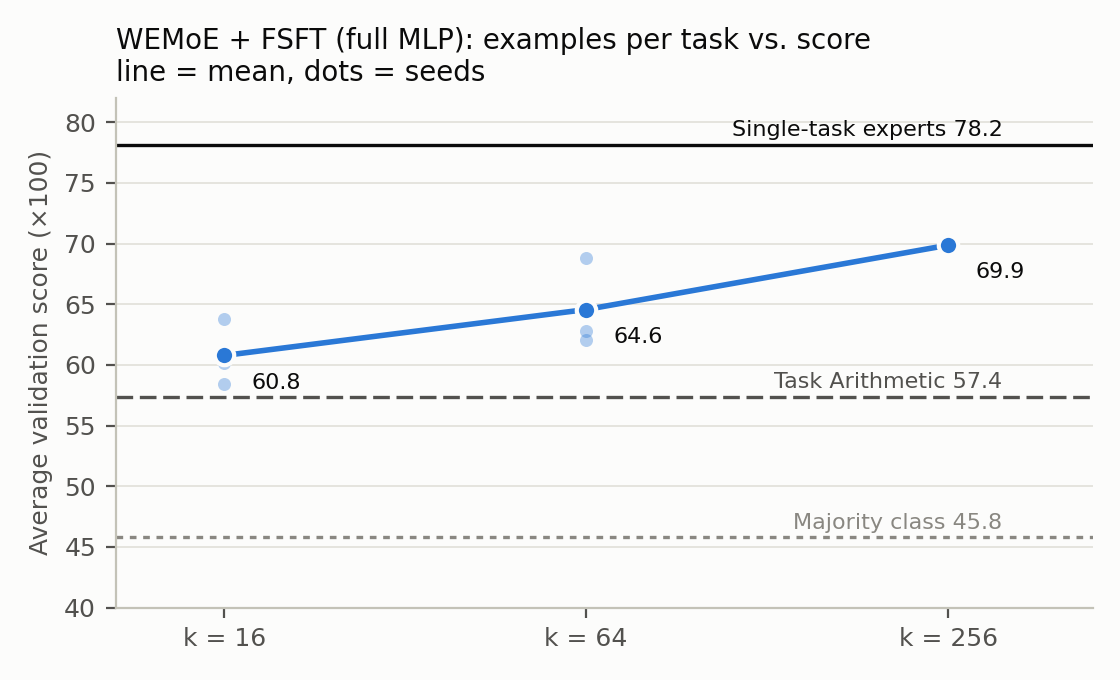
\includegraphics[width=.4\linewidth]{k_sweep.png}
  \caption{Điểm trung bình trên tập kiểm định của WEMoE full MLP theo ngân sách few-shot. Đường là giá trị trung bình, các chấm là từng seed.}
  \label{fig:k-sweep}
\end{figure}

\section{Hành vi định tuyến}
\label{sec:routing}

Hình~\ref{fig:routing} cho thấy giá trị trung bình của bộ định tuyến theo lớp và tác vụ đầu vào của một mô hình đã huấn luyện. Nhiều giá trị nằm xa giá trị ban đầu khoảng $\lambda$, và có cả hai dấu, điều mà một tổ hợp lồi không thể biểu diễn. Các ô trông khá giống nhau, nên phần lớn mẫu hình được chia sẻ giữa các tác vụ đầu vào, dù chúng cũng khác nhau ở một số chỗ, cho thấy định tuyến phụ thuộc một phần vào đầu vào. Trong mô hình này, cột của chuyên gia RTE mang giá trị âm ở hai lớp cuối với mọi loại đầu vào.

\begin{figure}[htbp]
  \centering
  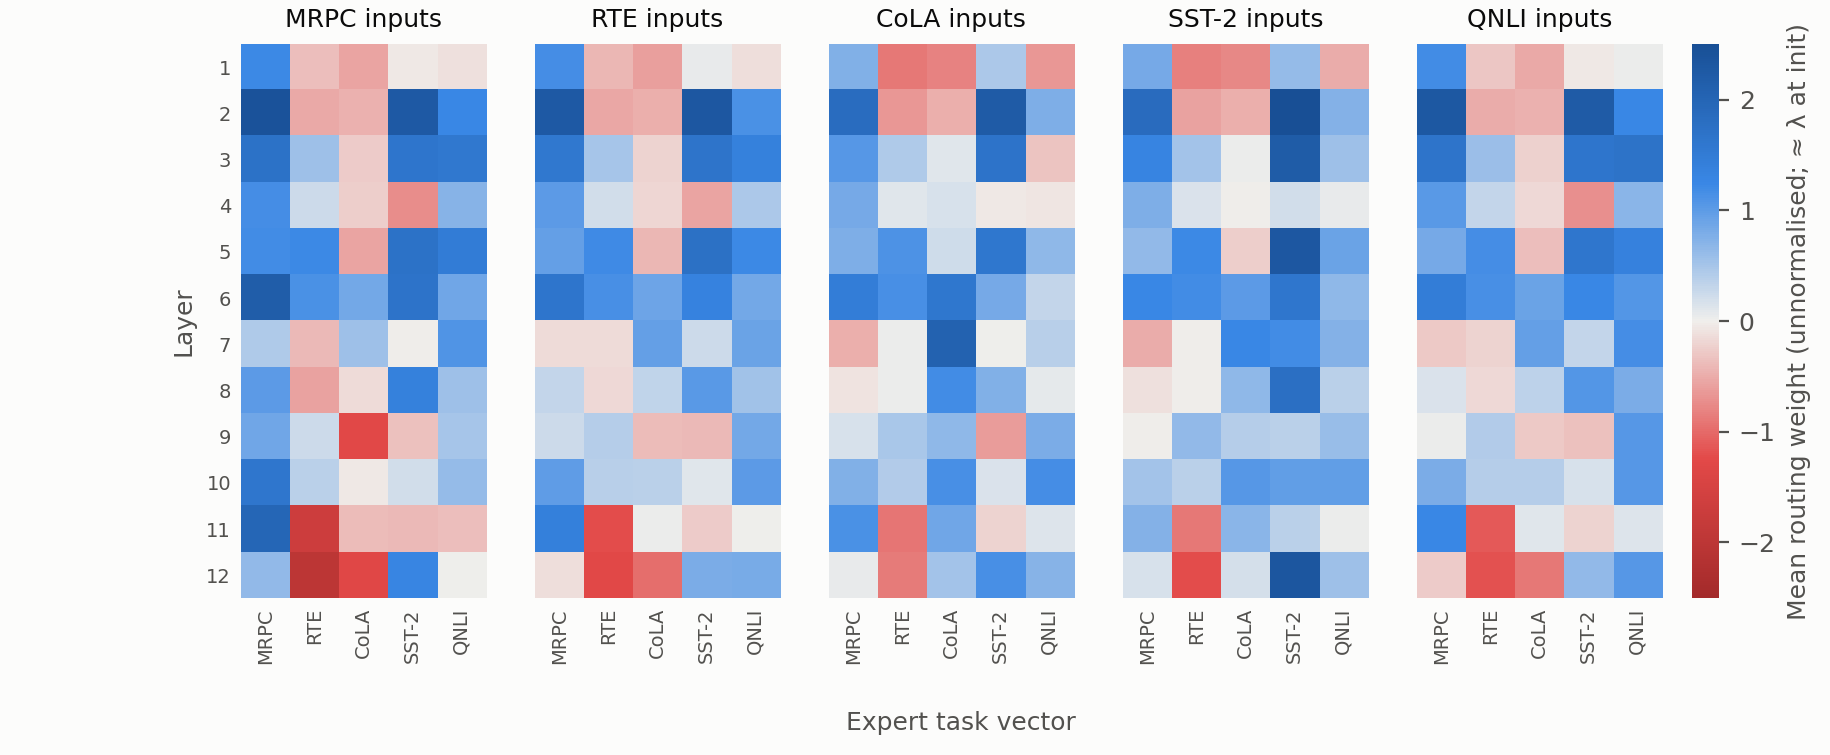
\includegraphics[width=.6\linewidth]{routing_clean.png}
  \caption{Giá trị trung bình của bộ định tuyến theo lớp và tác vụ đầu vào (full MLP, $k=256$, seed 0). Màu xanh cộng và màu đỏ trừ một véc-tơ tác vụ.}
  \label{fig:routing}
\end{figure}

Chúng tôi định lượng mẫu hình này từ giá trị bộ định tuyến của từng mẫu kiểm định. Với seed 0, các giá trị riêng lẻ trải từ $-3.0$ đến $4.4$, và tổng theo lớp của các giá trị trung bình trên toàn bộ mẫu đạt 5.8, so với 1.5 lúc khởi tạo. Ma trận định tuyến trung bình của các tác vụ đầu vào khác nhau có tương quan trung bình 0.82 (0.84 với seed 1 và 2), trong khi tác vụ đầu vào giải thích khoảng 58\% phương sai định tuyến (60\% với seed 1 và 2). Bảng~\ref{tab:own} cho thấy phần lớn các tác vụ tăng trọng số cho chuyên gia của chính mình, trừ RTE.

Chuyên gia RTE hành xử khác nhau giữa hai phạm vi, và một seed là chưa đủ để đọc khác biệt này. Giá trị của nó trên đầu vào RTE ở lớp 12 mang dấu âm với full MLP ở cả ba seed ($-1.28$, $-0.65$, $-0.76$) và dấu dương với intermediate-only ($2.04$, $1.16$, $1.53$). Giá trị trung bình theo lớp kém ổn định hơn: với intermediate-only, nó là 0.96, 0.27 và 0.31, trong khi độ chính xác RTE nằm trong khoảng 58.1 đến 59.9, nên trung bình này không giải thích được kết quả RTE. Bằng chứng này chỉ cho thấy mối liên hệ và không xác lập vì sao RTE thất bại.

\begin{table}[htbp]
  \centering\tablestyle
  \caption{Giá trị trung bình của bộ định tuyến dành cho chuyên gia của chính tác vụ, lấy trung bình qua các lớp (full MLP, $k=256$, seed 0).}
  \label{tab:own}
  \begin{tabular}{l c c c c c}
    \toprule
    & MRPC & SST-2 & QNLI & CoLA & RTE\\
    \midrule
    Trên đầu vào của chính nó & 1.37 & 1.37 & 0.94 & 0.61 & 0.01\\
    Trên đầu vào của tác vụ khác & 0.77 & 0.67 & 0.56 & $-0.02$ & $-0.01$\\
    \bottomrule
  \end{tabular}
\end{table}

\section{Lưu trữ, số tham số và độ trễ suy luận}
\label{sec:efficiency}

Bảng~\ref{tab:storage} phân tách các tham số được lưu, khớp với Phương trình~\eqref{eq:storage} và được đo trên các mô hình đã dựng. Véc-tơ tác vụ chiếm ưu thế, với 283.3M trong 400.0M tham số của mô hình full MLP.

\begin{table}[htbp]
  \centering\tablestyle
  \caption{Số tham số lưu trữ (triệu) theo thành phần, và tổng dung lượng ở độ chính xác 32-bit.}
  \label{tab:storage}
  \setlength{\tabcolsep}{4pt}\begin{tabular}{l r r r r r r r r}
    \toprule
    Triển khai & Tĩnh & MLP gốc & Véc-tơ tác vụ & Định tuyến & Head & Tổng & GiB & So với 5 MH\\
    \midrule
    5 mô hình riêng & -- & -- & -- & -- & -- & 547.4 & 2.04 & 100.0\%\\
    Task Arithmetic & -- & -- & -- & -- & -- & 109.5 & 0.41 & 20.0\%\\
    WEMoE, full MLP & 52.8 & 56.7 & 283.3 & 7.13 & 0.008 & 400.0 & 1.49 & 73.1\%\\
    WEMoE, intermediate-only & 81.1 & 28.3 & 141.7 & 7.13 & 0.008 & 258.4 & 0.96 & 47.2\%\\
    \bottomrule
  \end{tabular}
\end{table}

Bảng~\ref{tab:latency} báo cáo độ trễ trên một GPU T4, với các token id ngẫu nhiên dài 128, mixed precision và head MRPC, là trung bình của 10 lượt truyền xuôi sau 3 lượt khởi động. Dòng mô hình riêng đo một chuyên gia, vì mỗi đầu vào sẽ đi đến đúng chuyên gia của nó theo mã tác vụ. Số liệu batch 1 chỉ mang tính tham khảo: chúng lệch tới 27\% giữa hai lần đo (24.05 ms và 18.90 ms với mô hình intermediate-only), trong khi số liệu batch 32 khớp trong khoảng 5\%. Ở batch 32, mô hình full MLP chậm hơn một BERT khoảng 4.5 lần và mô hình intermediate-only khoảng 2.9 lần, và mô hình full MLP cần khoảng 2.8 lần bộ nhớ GPU cao nhất.

\begin{table}[htbp]
  \centering\tablestyle
  \caption{Độ trễ suy luận và bộ nhớ GPU cao nhất trên một T4, từ lần đo cuối. $^{*}$Đo một chuyên gia.}
  \label{tab:latency}
  \begin{tabular}{l c c c c}
    \toprule
    & \multicolumn{2}{c}{Batch 1} & \multicolumn{2}{c}{Batch 32}\\
    Triển khai & ms/mẫu & MB cao nhất & ms/mẫu & MB cao nhất\\
    \midrule
    BERT riêng theo tác vụ$^{*}$ & 11.64 & 614 & 1.61 & 704\\
    Task Arithmetic & 12.67 & 435 & 1.63 & 519\\
    WEMoE, full MLP & 27.83 & 1615 & 7.31 & 1987\\
    WEMoE, intermediate-only & 18.90 & 1061 & 4.69 & 1387\\
    \bottomrule
  \end{tabular}
\end{table}

\chapter{Đánh đổi và thảo luận}
\label{ch:discussion}

\section{Những gì kết quả chứng minh}

Các phép đo cho thấy ba điều trong bối cảnh này. Hợp nhất tĩnh gần với dự đoán hằng trên hai tác vụ nhỏ nhất. Các bộ định tuyến huấn luyện trên 256 mẫu mỗi tác vụ nâng điểm trung bình thêm 12.5 điểm và mức tăng so với lớp đa số từ 18.4 lên 59.1. Các hệ số cố định huấn luyện trên cùng dữ liệu chỉ cải thiện điểm trung bình 1 điểm.

Diễn giải của chúng tôi là định tuyến phụ thuộc đầu vào đóng góp phần lớn cải thiện so với Task Arithmetic. Diễn giải này vượt quá phép đo trực tiếp, vì hai biến thể còn khác nhau về sức chứa (7.1M so với 60 tham số) và learning rate, và ablation chỉ được thử với một learning rate, dù điểm dev tốt nhất của nó chỉ thay đổi 0.2.

\section{Đánh đổi giữa độ chính xác, tham số/lưu trữ và độ trễ}

WEMoE full MLP và intermediate-only đạt điểm trung bình tương tự (69.9 và 69.1), nhưng thất bại ở các tác vụ khác nhau. Intermediate-only lưu 47.2\% tham số của năm mô hình, nhỏ hơn biến thể full 35\%, huấn luyện nhanh gấp khoảng hai lần (8.4 so với 16.3 phút mỗi lần chạy) và suy luận nhanh hơn. Full MLP có mức tăng cao hơn (59.1 so với 54.8), dù khoảng cách 0.8 điểm ở điểm trung bình nằm trong mức nhiễu lấy mẫu.

Lưu ít tham số hơn không có nghĩa là suy luận nhanh hơn. Cả hai biến thể WEMoE lưu ít hơn năm chuyên gia nhưng lại chậm hơn trên mỗi mẫu, vì mỗi mẫu có trọng số hợp nhất riêng và không thể dùng chung một phép nhân ma trận trong batch. Task Arithmetic nhỏ nhất (20\%) và có tốc độ như một BERT, nhưng điểm thấp hơn WEMoE full MLP 12.5 điểm.

\section{Ý nghĩa thực tiễn}

Mỗi đầu vào trong thiết lập này đều đi kèm mã tác vụ, nên năm chuyên gia có thể được chọn trực tiếp theo tác vụ. Chúng chính xác hơn WEMoE full MLP trên mọi tác vụ, nhanh hơn trên mỗi mẫu và chỉ lớn hơn khoảng 37\%. Khi đã biết mã tác vụ và dung lượng cho phép, các chuyên gia vẫn là lựa chọn tốt hơn trong thực nghiệm này. WEMoE chủ yếu đáng cân nhắc khi cần giảm lưu trữ, và trường hợp này mạnh nhất với biến thể intermediate-only. Các bối cảnh không có mã tác vụ tường minh có thể có lợi hơn cho nó, nhưng mô hình hợp nhất ở đây vẫn dùng mã tác vụ để chọn head, và các bối cảnh đó chưa được đánh giá. Cũng không nên chỉ đọc điểm trung bình, vì nó che khuất những thất bại ở mức tác vụ mà mốc lớp đa số làm lộ ra.

\section{Hạn chế, nguy cơ đối với tính hợp lệ và câu hỏi còn mở}

\begin{itemize}
  \item \textbf{Tính hợp lệ nội tại.} ``Few-shot'' chưa nghiêm ngặt theo nghĩa của Perez và cộng sự~\cite{perez2021truefewshot}, vì nhãn dùng để lựa chọn cũng phải được tính: ở $k=256$, FSFT huấn luyện trên tổng cộng 1\,280 mẫu có nhãn, trong khi việc lựa chọn dùng 3\,471 mẫu dev. Điểm dev của SST-2 cũng đánh giá cao hơn thực tế chất lượng mô hình hợp nhất (Mục~\ref{sec:merging}).
  \item \textbf{Tính hợp lệ thống kê.} Độ lệch chuẩn bao gồm ba seed FSFT và không tính biến thiên của các chuyên gia và cách chia dữ liệu, vốn chỉ dùng một seed. RTE và MRPC có tập kiểm định nhỏ, với sai số chuẩn khoảng 3 và 2 điểm, lớn hơn một số khác biệt được thảo luận, kể cả 52.0 so với 52.7 trên RTE.
  \item \textbf{Tính hợp lệ bên ngoài.} Kết quả đến từ một lần chạy đầy đủ trên năm tác vụ nhị phân với một backbone, và không nên khái quát ra ngoài thiết lập này. Backbone, tác vụ, hàm mục tiêu và dữ liệu đều khác với Tang và cộng sự~\cite{tang2024wemoe}, nên mọi so sánh với nghiên cứu đó chỉ mang tính định tính.
  \item \textbf{Tính hợp lệ của cấu trúc đo.} Điểm trung bình trộn lẫn accuracy, F1 và MCC. Độ trễ dùng đầu vào ngẫu nhiên trên một GPU, và số liệu batch 1 dao động giữa các lần đo. Các số liệu định tuyến chỉ cho thấy mối liên hệ, và một số trong đó dao động giữa các seed.
\end{itemize}

Các câu hỏi còn mở gồm vì sao RTE thất bại với full MLP, biến thiên định tuyến trong cùng một tác vụ đi theo yếu tố nào, và điểm còn tăng bao xa khi vượt quá $k=256$.

\section{Phát hiện đã chứng minh và giả thuyết còn mở}

Bảng~\ref{tab:findings} tách những gì phép đo xác lập trong bối cảnh này khỏi những gì còn phải kiểm chứng.

\begin{table}[htbp]
  \centering\tablestyle
  \caption{Phát hiện đã chứng minh và giả thuyết còn mở.}
  \label{tab:findings}
  \begin{tabularx}{\linewidth}{*{2}{>{\raggedright\arraybackslash}X}}
    \toprule
    Đã chứng minh trong bối cảnh này & Giả thuyết còn mở\\
    \midrule
    FSFT với bộ định tuyến cải thiện rõ rệt so với Task Arithmetic về trung bình. & Tính phụ thuộc đầu vào, chứ không phải sức chứa, giải thích phần lớn cải thiện này.\\
    Hệ số cố định với các thiết lập đã thử gần như không cải thiện. & Một learning rate khác sẽ không thay đổi kết quả này.\\
    Ngân sách nhỏ không ổn định; điểm trung bình vẫn tăng ở $k=256$. & Ngân sách lớn hơn sẽ tiếp tục nâng điểm.\\
    Hai phạm vi yếu ở các tác vụ khác nhau. & Thất bại ở RTE bắt nguồn từ đánh đổi trong hàm mục tiêu tổng và việc chọn theo điểm trung bình, hoặc từ chuyên gia RTE yếu.\\
    Intermediate-only đạt bước tốt nhất muộn (400--500 trên 500). & Thêm bước sẽ cải thiện mô hình intermediate-only.\\
    \bottomrule
  \end{tabularx}
\end{table}

\chapter{Kết luận và hướng phát triển}
\label{ch:conclusion}

\section{Trả lời các câu hỏi nghiên cứu}

\paragraph{RQ1.} Với 256 mẫu có nhãn mỗi tác vụ, các bộ định tuyến nâng điểm trung bình từ 57.4 lên $69.9\pm0.1$ và mức tăng so với lớp đa số từ 18.4\% lên 59.1\%. Khoảng cách rõ rệt với các chuyên gia (78.2) vẫn còn.

\paragraph{RQ2.} Điểm trung bình tăng từ 60.8 ở $k=16$ lên 64.6 ở $k=64$ và 69.9 ở $k=256$, và chưa chững lại. Ngân sách nhỏ không ổn định giữa các seed.

\paragraph{RQ3.} Các hệ số cố định chỉ đạt 58.4, nên riêng các hệ số tĩnh tốt hơn không giải thích được cải thiện, dù ablation chưa tách được tính phụ thuộc đầu vào khỏi sức chứa.

\paragraph{RQ4.} Nâng cấp full MLP và intermediate-only đạt điểm trung bình tương tự với các thất bại khác nhau, lần lượt ở RTE và MRPC. Intermediate-only cần 47.2\% dung lượng của năm mô hình, so với 73.1\%. Ở batch 32, intermediate-only và full MLP chậm hơn một BERT khoảng 2.9 và 4.5 lần.

\section{Đánh giá các mục tiêu}

Bảng~\ref{tab:goals} đánh giá các mục tiêu ở Mục~\ref{sec:problem} dựa trên bằng chứng.

\begin{table}[htbp]
  \centering\tablestyle
  \caption{Các mục tiêu của bài toán so với kết quả.}
  \label{tab:goals}
  \begin{tabularx}{\linewidth}{>{\raggedright\arraybackslash}p{3.2cm} X >{\raggedright\arraybackslash}p{5.2cm}}
    \toprule
    Mục tiêu & Bằng chứng & Đánh giá\\
    \midrule
    O1. Tích hợp động & Trọng số MLP theo từng đầu vào; hệ số cố định đạt 58.4, so với 69.9 & Đạt theo thiết kế; đóng góp của tính phụ thuộc đầu vào được ủng hộ nhưng chưa được tách riêng\\
    O2. Gần các mô hình riêng theo tác vụ & 69.9 so với 78.2, mức tăng 59.1\%; RTE và MRPC vẫn yếu; không tác vụ nào đạt mức chuyên gia & Đạt một phần\\
    O3. Ít tham số lưu trữ hơn & 73.1\% (full MLP) hoặc 47.2\% (intermediate-only) của năm mô hình & Đạt, đổi lại độ trễ cao hơn\\
    \bottomrule
  \end{tabularx}
\end{table}

\section{Đóng góp chính và ý nghĩa thực tiễn}

Đóng góp mang tính thực tiễn, và không có thuật toán mới nào được đề xuất. Nghiên cứu này chuyển WEMoE sang encoder BERT chuẩn hóa sau với định tuyến có tính đến mặt nạ attention, áp dụng quy trình tách biệt dữ liệu của từng giai đoạn, và đánh giá hai phạm vi nâng cấp, ba ngân sách nhãn và một ablation không phụ thuộc đầu vào so với mốc lớp đa số. Trong thực tế, hợp nhất phụ thuộc đầu vào vượt rõ rệt hợp nhất tĩnh về trung bình nhưng không vượt các chuyên gia riêng theo tác vụ, và lý do dùng nó chủ yếu nằm ở ràng buộc lưu trữ.

\section{Hướng phát triển}

Hợp nhất bốn tác vụ không có RTE sẽ kiểm tra liệu RTE có can nhiễu các tác vụ khác không. Ngân sách lớn hơn ($k=512$ và $1024$) sẽ cho thấy điểm có chững lại không, và thêm bước FSFT sẽ kiểm tra biến thể intermediate-only. Đo chuẩn của véc-tơ tác vụ theo từng loại mô-đun sẽ kiểm chứng lý do nâng cấp MLP trên BERT. Một quy trình nghiêm ngặt sẽ giới hạn dev ở $k$, và thêm seed cho các chuyên gia và cách chia dữ liệu sẽ cho ước lượng đáng tin cậy hơn. Phân tích theo từng mẫu sẽ cho thấy biến thiên định tuyến trong một tác vụ đi theo yếu tố nào.


\clearpage
\phantomsection
\addcontentsline{toc}{chapter}{Tài liệu tham khảo}
{\small\def\baselinestretch{1.0}\selectfont\setlength{\bibsep}{2pt}
\bibliographystyle{plainnat}
\bibliography{references_v3}}
\end{document}
